\documentclass[aspectratio=169]{beamer}
\usetheme{Madrid}
\usecolortheme{default}
\usepackage[utf8]{inputenc}
\usepackage[T5]{fontenc}
\usepackage{graphicx}
\usepackage{hyperref}
\usepackage{booktabs}

\setbeamertemplate{caption}[numbered]
\renewcommand{\figurename}{Hình}
\renewcommand{\thefigure}{1.\arabic{figure}}

\title[Chương 1: Khái niệm Học sâu]{Học Sâu (Deep Learning) \\ \vspace{0.5cm} \Large Chương 1: Khái niệm Học sâu}
\author{Đại học Đông Á}
\date{\today}

\begin{document}

\begin{frame}
    \titlepage
\end{frame}

\begin{frame}{Nội dung chương}
    \tableofcontents
\end{frame}

% ==============================
\section{1. Giới thiệu và Các khái niệm cơ bản}
% ==============================

\begin{frame}{Sự bùng nổ của Trí tuệ Nhân tạo (AI)}
    \begin{itemize}
        \item \textbf{Truyền thông và thực tế:} AI xuất hiện ở khắp nơi trong thập kỷ qua. Chúng ta được hứa hẹn về một tương lai với chatbot thông minh, xe tự lái và trợ lý ảo.
        \item \textbf{Sự phân cực trong góc nhìn:}
        \begin{itemize}
            \item Một số cho rằng tương lai u ám: máy móc sẽ cướp đi công việc của con người.
            \item Một số cho rằng tương lai không tưởng (utopian): năng suất tăng gấp hàng trăm lần, không ai cần phải làm việc.
        \end{itemize}
        \item \textbf{Mục tiêu của chương này:} Nhận biết "tín hiệu" giữa "tiếng ồn". Tìm hiểu những gì AI và Học sâu thực sự đã đạt được, giới hạn của chúng, và định hướng phát triển thực tế trong tương lai.
    \end{itemize}
\end{frame}

\begin{frame}{Trí tuệ nhân tạo, Máy học và Học sâu}
    \begin{columns}
        \column{0.5\textwidth}
        \begin{itemize}
            \item \textbf{Trí tuệ nhân tạo (AI):} Lĩnh vực bao trùm, nỗ lực tự động hóa các công việc trí tuệ của con người.
            \item \textbf{Học máy (Machine Learning - ML):} Một nhánh của AI, hệ thống tự động học cấu trúc từ dữ liệu.
            \item \textbf{Học sâu (Deep Learning - DL):} Một nhánh của Học máy, tập trung học các biểu diễn thông qua vô số lớp liên tiếp.
        \end{itemize}
        
        \column{0.5\textwidth}
        \begin{figure}
            \centering
            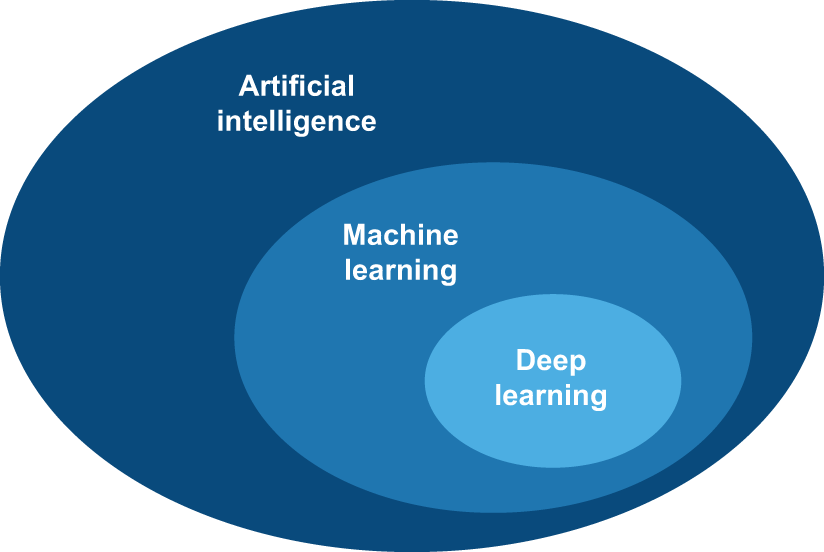
\includegraphics[width=\textwidth,height=0.8\textheight,keepaspectratio]{../../images/ch01/ai-ml-dl.07201556.png}
            \caption{Mối quan hệ giữa AI, ML và DL}
        \end{figure}
    \end{columns}
\end{frame}

\begin{frame}{Lịch sử Trí tuệ Nhân tạo}
    \begin{itemize}
        \item \textbf{Sự khởi đầu:} Ra đời vào những năm 1950 khi các nhà tiên phong đặt câu hỏi liệu máy tính có thể "suy nghĩ" được hay không.
        \item \textbf{Hội thảo Dartmouth (1956):} John McCarthy tổ chức một hội thảo nghiên cứu và thuật ngữ \textit{Trí tuệ Nhân tạo (Artificial Intelligence)} chính thức được kết tinh.
        \item \textbf{Mục tiêu ban đầu:}
        \begin{itemize}
            \item Mô phỏng khía cạnh học tập và các đặc điểm của trí thông minh.
            \item Sử dụng ngôn ngữ, hình thành khái niệm trừu tượng.
            \item Giải quyết các vấn đề vốn chỉ dành cho con người.
        \end{itemize}
    \end{itemize}
\end{frame}

\begin{frame}{AI Cổ điển (Symbolic AI)}
    \begin{itemize}
        \item \textbf{Định nghĩa:} Kỷ nguyên từ 1950 - 1980. Con người lập trình ra một bộ vô số các quy tắc logic tường minh để thao tác kiến thức.
        \item \textbf{Hệ chuyên gia (Expert Systems):} Đạt đỉnh cao phổ biến vào những năm 1980. Mô hình hóa kiến thức của con người dưới dạng tập luật (If-Then).
        \item \textbf{Thành công:} Rất phù hợp để giải quyết các vấn đề logic và được xác định rõ ràng, ví dụ như chơi cờ vua.
    \end{itemize}
\end{frame}

\begin{frame}{Hạn chế của AI Cổ điển}
    \begin{block}{Tại sao Symbolic AI dần bộc lộ giới hạn?}
        Mặc dù có khả năng chơi cờ xuất sắc, nhưng hệ thống lại thất bại trước các vấn đề thực tế, mơ hồ và ít tính cấu trúc hơn.
    \end{block}
    \begin{itemize}
        \item Không thể viết ra một bộ quy tắc logic tường minh cho các tác vụ như:
        \begin{itemize}
            \item \textbf{Phân loại hình ảnh} (nhận dạng chó, mèo).
            \item \textbf{Nhận dạng giọng nói} (chuyển âm thanh thành văn bản).
            \item \textbf{Dịch ngôn ngữ tự nhiên} (hiểu ngữ cảnh để dịch).
        \end{itemize}
        \item Từ đó, một hướng tiếp cận mới cần được nảy sinh để giải quyết vấn đề của AI cổ điển: \textbf{Học Máy (Machine Learning)}.
    \end{itemize}
\end{frame}

\begin{frame}{Học máy (Machine Learning) - Nguồn gốc}
    \begin{itemize}
        \item \textbf{Ada Lovelace và Máy phân tích (1840s):} Máy phân tích (của Charles Babbage) chỉ được cho là xử lý cơ học những gì con người thiết lập. Lovelace từng cho rằng "máy móc không có ý định tạo ra bất cứ thứ gì".
        \item \textbf{Alan Turing (1950):} Trong bài báo \textit{"Máy tính và Trí thông minh"}, Turing đã đưa ra khái niệm \textbf{Turing Test} và khiêu khích ý tưởng rằng máy tính có thể mô phỏng trí tuệ con người, thậm chí có khả năng học tập (đi ngược lại quan điểm của Ada Lovelace).
    \end{itemize}
\end{frame}

\begin{frame}{Mô hình Lập trình Mới}
    \begin{columns}
        \column{0.45\textwidth}
        \textbf{Lập trình Cổ điển:}
        \begin{itemize}
            \item Con người thiết lập \textbf{Quy tắc (Rules)}.
            \item Dữ liệu đầu vào kết hợp với Quy tắc sẽ trả về \textbf{Câu trả lời}.
        \end{itemize}
        \vspace{0.5cm}
        \textbf{Học máy (Machine Learning):}
        \begin{itemize}
            \item Cung cấp \textbf{Dữ liệu} cùng \textbf{Câu trả lời dự kiến}.
            \item Hệ thống sẽ tự tìm ra \textbf{Quy tắc} ẩn sau dữ liệu.
        \end{itemize}
        
        \column{0.55\textwidth}
        \begin{figure}
            \centering
            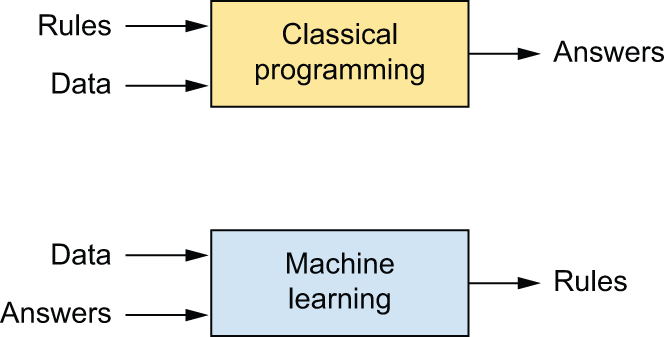
\includegraphics[width=\textwidth,height=0.8\textheight,keepaspectratio]{../../images/ch01/a-new-programming-paradigm.e8d1a1c2.png}
            \caption{Mô hình lập trình cổ điển vs. Học máy}
        \end{figure}
    \end{columns}
\end{frame}

\begin{frame}{Đặc điểm cốt lõi của Học máy}
    \begin{itemize}
        \item Một hệ thống Học máy không được lập trình tường minh, mà nó được \textbf{huấn luyện (trained)}.
        \item Hệ thống được cung cấp vô số ví dụ về một nhiệm vụ và tiến hành tìm ra \textbf{cấu trúc thống kê} trong các ví dụ đó.
        \item Khác với Phân tích thống kê Bayesian cổ điển: Học máy có khả năng xử lý tập dữ liệu khổng lồ, phức tạp (ví dụ: một bức ảnh có hàng chục ngàn pixel).
        \item Học máy, đặc biệt là Học sâu, mang tính ứng dụng kỹ thuật (engineering) nhiều hơn là lý thuyết toán học thuần túy.
    \end{itemize}
\end{frame}

% ==============================
\section{2. Học biểu diễn và Học quy tắc từ dữ liệu}
% ==============================

\begin{frame}{Ba yếu tố thiết yếu của Học máy}
    Để một hệ thống học máy có thể khám phá ra quy tắc từ dữ liệu, chúng ta cần:
    \begin{enumerate}
        \item \textbf{Điểm dữ liệu đầu vào (Input data):} Ví dụ, file âm thanh giọng nói, hoặc hình ảnh chứa vật thể cần nhận dạng.
        \item \textbf{Đầu ra dự kiến (Expected output / Targets):} Ví dụ, văn bản (transcript) ghi lại lời nói, hoặc nhãn "chó/mèo" cho hình ảnh.
        \item \textbf{Cách đo lường hiệu suất (Feedback / Loss):} Một đại lượng đánh giá khoảng cách giữa kết quả dự đoán của thuật toán so với đầu ra dự kiến thực tế. 
    \end{enumerate}
    $\rightarrow$ Thuật toán sử dụng tín hiệu phản hồi này để \textbf{điều chỉnh} hành vi. Bước điều chỉnh chính là \textbf{quá trình học tập}.
\end{frame}

\begin{frame}{Học biểu diễn (Learning representations)}
    \begin{itemize}
        \item Vấn đề trung tâm của Học máy là \textbf{chuyển đổi dữ liệu một cách có ý nghĩa}.
        \item Mô hình học máy cố gắng tìm kiếm một biểu diễn (representation) mới, hữu ích hơn cho tác vụ.
        \item \textbf{Ví dụ thực tế:}
        \begin{itemize}
            \item Nếu bạn muốn yêu cầu "chọn tất cả các điểm ảnh màu đỏ", việc biểu diễn ảnh ở dạng \textbf{RGB} sẽ đơn giản hơn.
            \item Nếu bạn muốn yêu cầu "giảm độ bão hòa màu của ảnh", biểu diễn ở dạng \textbf{HSV} lại trực quan và dễ thao tác hơn nhiều.
        \end{itemize}
    \end{itemize}
\end{frame}

\begin{frame}{Ví dụ trực quan về Biểu diễn Không gian}
    \begin{columns}
        \column{0.5\textwidth}
        \begin{itemize}
            \item Giả sử chúng ta có các điểm trắng và đen trong một không gian tọa độ 2 chiều (x, y).
            \item Nhiệm vụ: Phân loại một điểm (x, y) bất kỳ là màu đen hay trắng.
            \item Trong hệ trục ban đầu, việc phân tách hai lớp này gặp khó khăn vì chúng nằm lộn xộn.
        \end{itemize}
        
        \column{0.5\textwidth}
        \begin{figure}
            \centering
            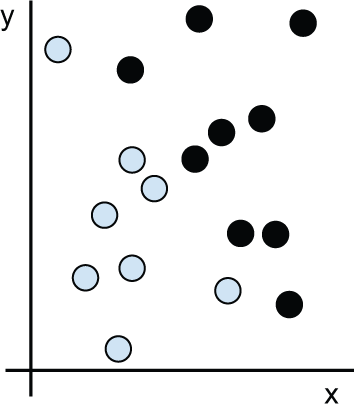
\includegraphics[width=\textwidth,height=0.8\textheight,keepaspectratio]{../../images/ch01/example_data_points.28a84f5a.png}
            \caption{Tọa độ các điểm đen và trắng (Dữ liệu gốc)}
        \end{figure}
    \end{columns}
\end{frame}

\begin{frame}{Biến đổi không gian tọa độ}
    \begin{columns}
        \column{0.45\textwidth}
        \begin{itemize}
            \item Chúng ta có thể dùng phép biến đổi toán học (thay đổi trục tọa độ).
            \item Trong không gian mới, bài toán trở nên vô cùng đơn giản:
            \begin{itemize}
                \item Điểm đen nằm ở khu vực $X > 0$.
                \item Điểm trắng nằm ở khu vực $X < 0$.
            \end{itemize}
            \item \textbf{Bài học:} Chuyển đổi biểu diễn làm thay đổi hoàn toàn mức độ phức tạp của bài toán gốc.
        \end{itemize}
        
        \column{0.55\textwidth}
        \begin{figure}
            \centering
            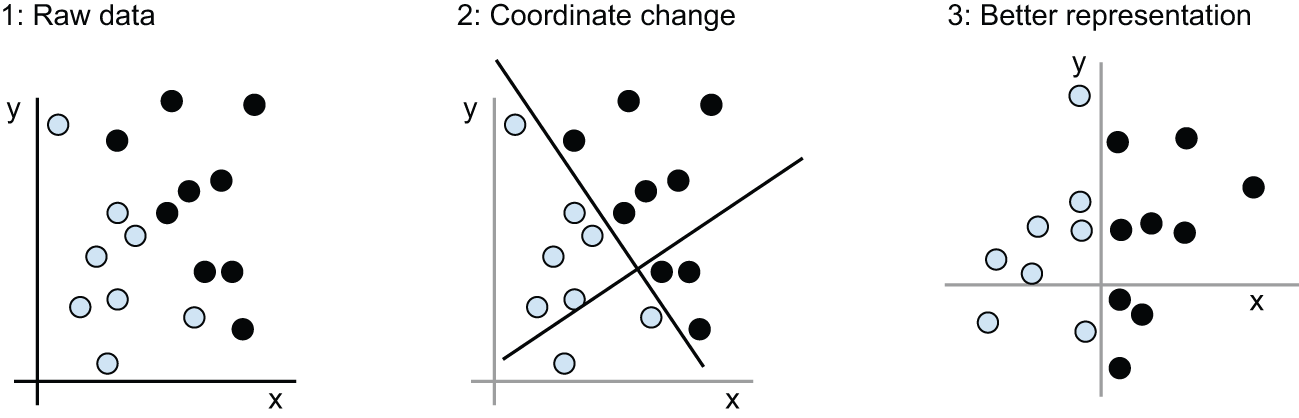
\includegraphics[width=\textwidth,height=0.8\textheight,keepaspectratio]{../../images/ch01/learning_representations.97fa3c4b.png}
            \caption{Sự thay đổi không gian giúp phân tách dữ liệu dễ dàng}
        \end{figure}
    \end{columns}
\end{frame}

\begin{frame}{Sự khó khăn của Trích xuất đặc trưng thủ công}
    \begin{itemize}
        \item Đối với bài toán điểm 2D, chúng ta có thể \textbf{thiết kế thủ công} (handcraft) sự biến đổi tọa độ.
        \item Nhưng với phân loại ảnh chữ số viết tay (có hàng ngàn pixel biến thiên) thì sao?
        \item Khái niệm \textbf{Feature Engineering (Kỹ thuật trích xuất đặc trưng):} Con người phải thiết lập các quy tắc như đếm số vòng lặp khép kín, phân tích biểu đồ cạnh (edges histogram)...
        \item \textbf{Yếu điểm:} Tốn rất nhiều thời gian, thiết kế cứng nhắc, rất dễ thất bại khi gặp các kiểu viết tay lạ.
    \end{itemize}
\end{frame}

\begin{frame}{Học tự động (Automated learning)}
    \begin{itemize}
        \item Thay vì thiết kế thủ công, ta cho phép hệ thống tìm kiếm tự động qua hàng triệu các phép biến đổi toán học.
        \item Tập hợp các phép biến đổi mà hệ thống có thể thử nghiệm được gọi là \textbf{Không gian giả thuyết (Hypothesis space)}.
        \item Học máy, bản chất là một quá trình tìm kiếm tự động trong không gian giả thuyết này, được hướng dẫn bởi điểm phản hồi (Loss), để tìm ra biểu diễn dữ liệu tốt nhất phục vụ cho việc giải quyết tác vụ.
    \end{itemize}
\end{frame}

% ==============================
\section{3. Sự "sâu" trong Học sâu}
% ==============================

\begin{frame}{Học sâu (Deep Learning) là gì?}
    \begin{itemize}
        \item Là một kỹ thuật mới trong Học máy nhằm tìm ra biểu diễn (representations).
        \item Chữ \textbf{"sâu" (deep)} ám chỉ ý tưởng về các lớp (layers) biểu diễn được xếp chồng liên tiếp nhau, ngày càng trở nên có tính tóm lược và ý nghĩa cao.
        \item \textbf{Độ sâu (Depth):} Là số lượng lớp đóng góp vào việc mô hình hóa dữ liệu (có thể lên tới hàng trăm hoặc hàng ngàn lớp).
        \item Các phương pháp Học máy cổ điển thường chỉ sử dụng 1 đến 2 bước chuyển đổi (được gọi là \textit{Học nông - Shallow learning}).
    \end{itemize}
\end{frame}

\begin{frame}{Mạng nơ-ron (Neural Network)}
    \begin{itemize}
        \item Các biểu diễn này được học bằng một mô hình có cấu trúc các tầng toán học xếp chồng nhau, gọi là \textbf{Mạng nơ-ron}.
        \item \textbf{Lưu ý về thuật ngữ:} Tên gọi xuất phát từ sinh học thần kinh, nhưng Học sâu hiện đại KHÔNG PHẢI là mô hình giả lập bộ não. 
        \item Không có bằng chứng cho thấy não bộ học bằng kỹ thuật lan truyền ngược (Backpropagation). Hãy coi Học sâu đơn thuần là một khung toán học phức tạp để biến đổi dữ liệu.
    \end{itemize}
\end{frame}

\begin{frame}{Quá trình chắt lọc thông tin qua các lớp}
    \begin{columns}
        \column{0.5\textwidth}
        Ví dụ: Phân loại chữ số viết tay (MNIST).
        \begin{itemize}
            \item Hình ảnh ban đầu là các mảng giá trị pixel.
            \item Mạng sâu hoạt động như một \textbf{hệ thống chắt lọc}.
            \item Khi dữ liệu đi qua các tầng, mạng bóc tách những thông tin không cần thiết và tinh lọc dần những đặc trưng quyết định (các nét thẳng, đường cong, vòng lặp...).
        \end{itemize}
        
        \column{0.5\textwidth}
        \begin{figure}
            \centering
            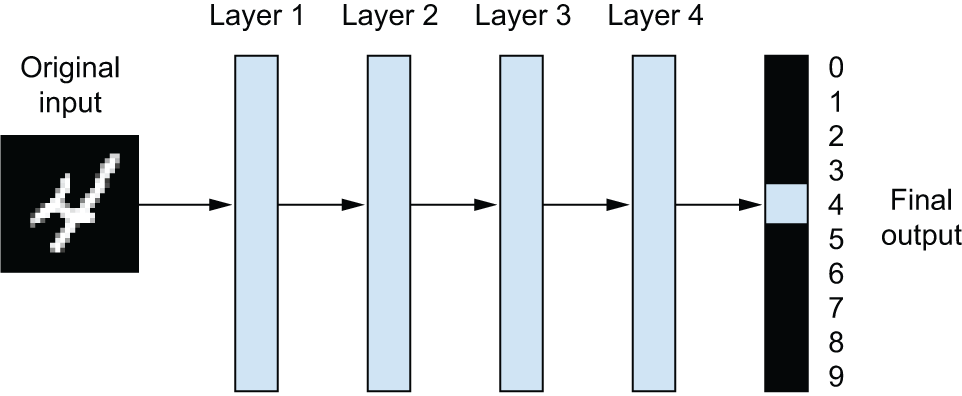
\includegraphics[width=\textwidth,height=0.8\textheight,keepaspectratio]{../../images/ch01/a_deep_network.32f0eedf.png}
            \caption{Cấu trúc Mạng nơ-ron sâu}
        \end{figure}
    \end{columns}
\end{frame}

\begin{frame}{Minh họa biểu diễn qua từng lớp}
    \begin{columns}
        \column{0.45\textwidth}
        \begin{itemize}
            \item \textbf{Layer 1:} Dữ liệu chưa rõ ràng.
            \item \textbf{Layer 2:} Các yếu tố hình học bắt đầu lộ diện.
            \item \textbf{Layer cuối cùng:} Mạng phân loại số một cách chính xác do biểu diễn của nó đã trở nên cực kỳ tinh lọc và tối ưu cho nhiệm vụ.
        \end{itemize}
        
        \column{0.55\textwidth}
        \begin{figure}
            \centering
            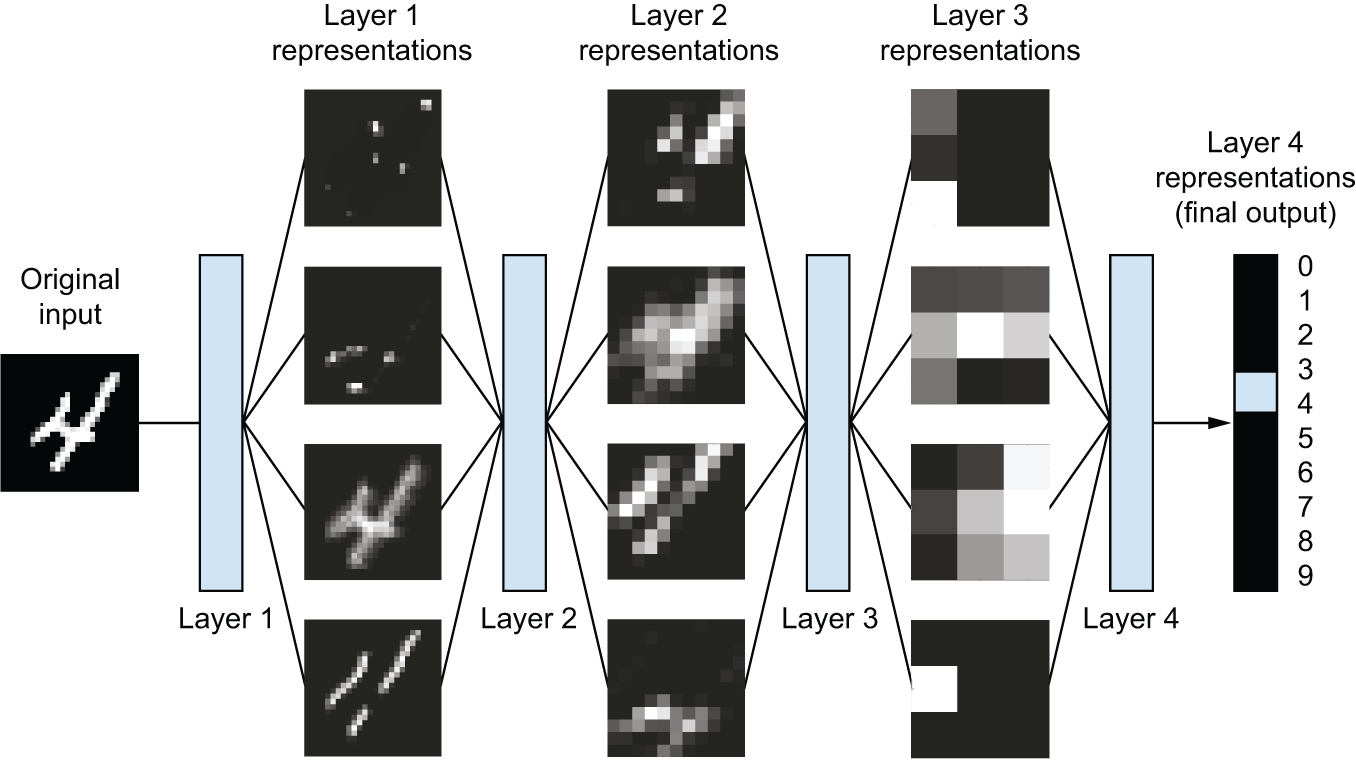
\includegraphics[width=\textwidth,height=0.8\textheight,keepaspectratio]{../../images/ch01/mnist_representations.fdb30a2d.png}
            \caption{Sự thay đổi biểu diễn qua các lớp}
        \end{figure}
    \end{columns}
\end{frame}

\begin{frame}{Điều gì làm Học sâu trở nên khác biệt?}
    Trước Học sâu, Học máy phụ thuộc rất lớn vào Kỹ thuật đặc trưng (Feature Engineering). 
    \begin{block}{Sức mạnh lớn nhất của Học Sâu}
        Học sâu \textbf{tự động hóa hoàn toàn} bước Feature Engineering. 
        Thay vì phải thiết kế thủ công nhiều khâu biến đổi dữ liệu một cách lắt léo, Học sâu học mọi đặc trưng chỉ trong một quá trình xuyên suốt (End-to-End).
    \end{block}
\end{frame}

\begin{frame}{Ba tính chất ưu việt của Học sâu}
    \begin{enumerate}
        \item \textbf{Sự đơn giản:} Loại bỏ quy trình tiền xử lý, rút trích tính năng phức tạp, gộp mọi thứ vào một đường ống duy nhất, thống nhất.
        \item \textbf{Khả năng mở rộng (Scalability):} Do đặc tính có thể huấn luyện theo các lô nhỏ (mini-batches) và dễ dàng song song hóa trên phần cứng mạnh như GPU, có thể xử lý tập dữ liệu khổng lồ vô hạn.
        \item \textbf{Tính linh hoạt và tái sử dụng:} Một mô hình có thể được tinh chỉnh liên tục mà không cần huấn luyện lại từ đầu. Các "Mô hình nền tảng" lớn (Foundation models) có thể được ứng dụng vào nhiều nhiệm vụ mới khác.
    \end{enumerate}
\end{frame}

% ==============================
\section{4. Cơ chế hoạt động của Mạng nơ-ron}
% ==============================

\begin{frame}{Thành phần cốt lõi của Mạng nơ-ron}
    \begin{columns}
        \column{0.5\textwidth}
        \begin{itemize}
            \item Các phép biến đổi dữ liệu tại một lớp được \textbf{tham số hóa (parameterized)} bởi một tập hợp các con số.
            \item Các con số này được gọi là \textbf{Trọng số (Weights)}.
            \item Việc "học" có nghĩa là tìm ra giá trị lý tưởng cho hàng triệu trọng số này, sao cho Input đi qua mạng sẽ ánh xạ chính xác ra Output.
        \end{itemize}
        
        \column{0.5\textwidth}
        \begin{figure}
            \centering
            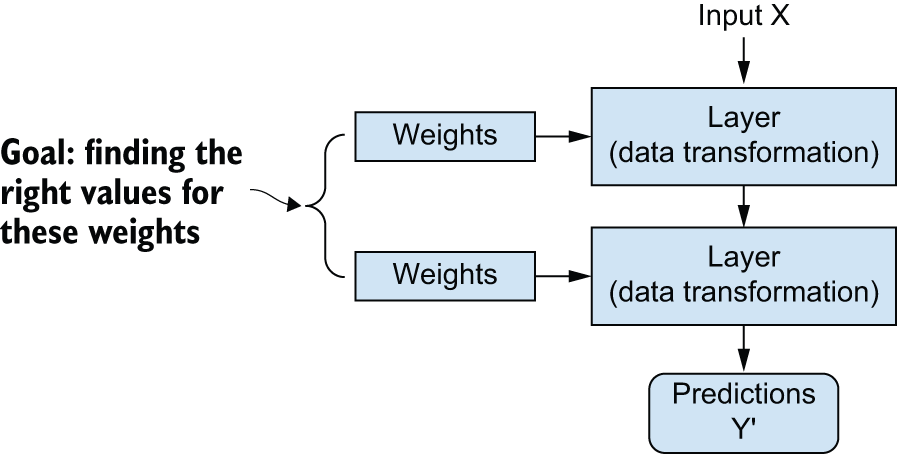
\includegraphics[width=\textwidth,height=0.8\textheight,keepaspectratio]{../../images/ch01/deep-learning-in-3-figures-1.55e5a910.png}
            \caption{Lớp nơ-ron và trọng số}
        \end{figure}
    \end{columns}
\end{frame}

\begin{frame}{Hàm mất mát (Loss Function)}
    \begin{columns}
        \column{0.5\textwidth}
        \begin{itemize}
            \item Để điều khiển được mạng, ta cần đo lường sự sai lệch giữa kết quả thực và kết quả dự đoán của mô hình.
            \item \textbf{Hàm mất mát (Loss Function)} nhận kết quả dự đoán và nhãn thực tế, rồi tính ra một "điểm số khoảng cách".
            \item Điểm số này càng thấp thì mạng dự đoán càng chính xác.
        \end{itemize}
        
        \column{0.5\textwidth}
        \begin{figure}
            \centering
            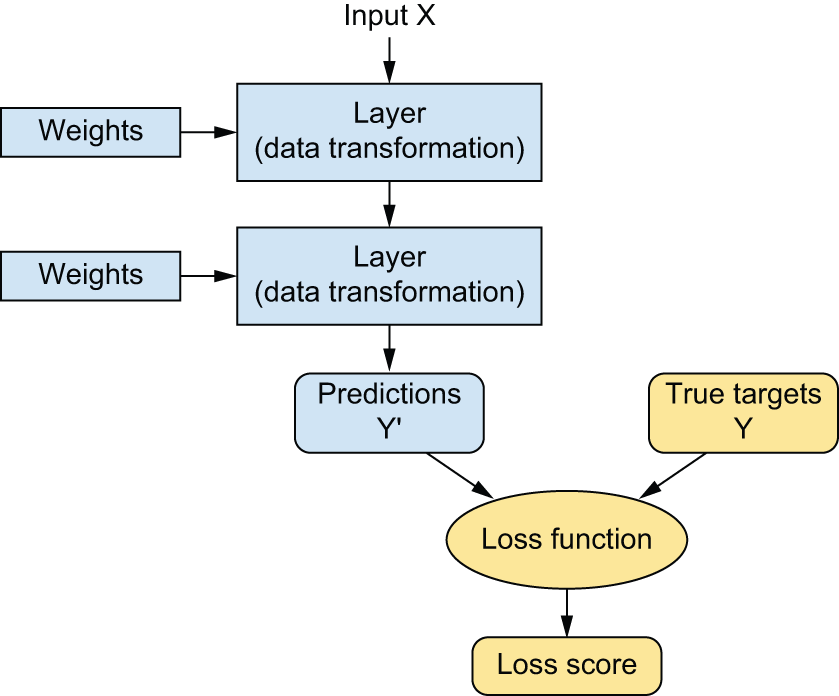
\includegraphics[width=\textwidth,height=0.8\textheight,keepaspectratio]{../../images/ch01/deep-learning-in-3-figures-2.bb3cebc2.png}
            \caption{Đo lường sai số bằng Loss Function}
        \end{figure}
    \end{columns}
\end{frame}

\begin{frame}{Tín hiệu phản hồi}
    \begin{itemize}
        \item Điểm số Loss Function chính là \textbf{tín hiệu phản hồi (feedback signal)} duy nhất để cải thiện chất lượng của mô hình.
        \item Tuy nhiên, với một mạng có hàng triệu tham số, việc thay đổi một trọng số có thể ảnh hưởng đến kết quả của tất cả các trọng số khác. Làm sao để biết nên tăng hay giảm từng trọng số?
        \item Chúng ta cần một hệ thống cập nhật có tính toán hướng tối ưu chính xác.
    \end{itemize}
\end{frame}

\begin{frame}{Bộ tối ưu hóa (Optimizer)}
    \begin{columns}
        \column{0.5\textwidth}
        \begin{itemize}
            \item Thủ thuật cơ bản trong Học sâu là sử dụng điểm Loss để đẩy bộ \textbf{Trọng số} đi theo hướng giúp giảm sai số.
            \item Việc này được thực hiện bởi \textbf{Bộ tối ưu hóa (Optimizer)}, áp dụng giải thuật cốt lõi: \textbf{Lan truyền ngược (Backpropagation)}.
            \item Backprop tính toán xem mỗi trọng số chịu trách nhiệm bao nhiêu phần trăm về sai số hiện tại.
        \end{itemize}
        
        \column{0.5\textwidth}
        \begin{figure}
            \centering
            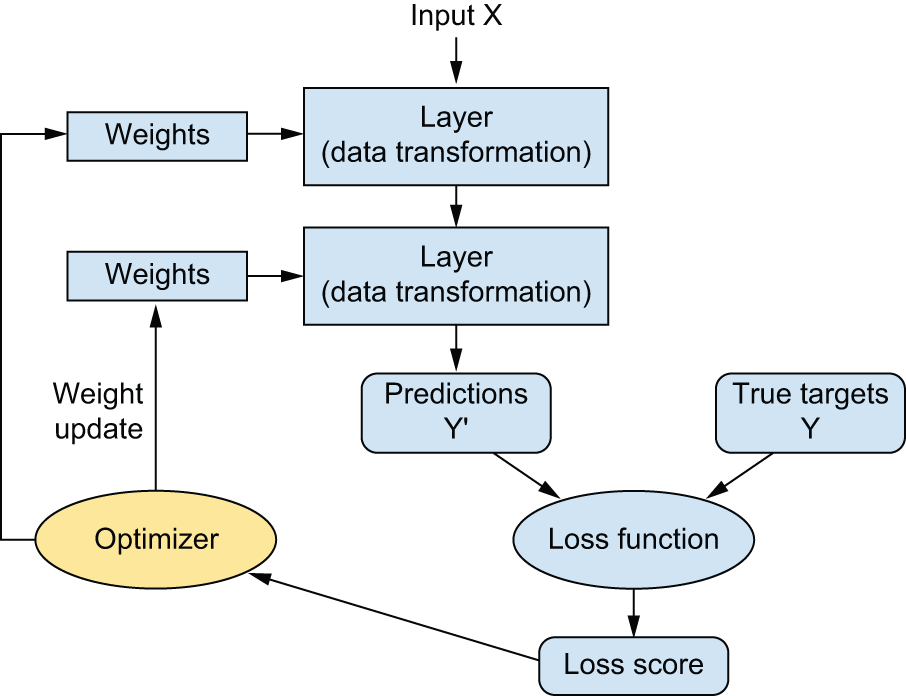
\includegraphics[width=\textwidth,height=0.8\textheight,keepaspectratio]{../../images/ch01/deep-learning-in-3-figures-3.de178fa4.png}
            \caption{Điều chỉnh trọng số qua Optimizer}
        \end{figure}
    \end{columns}
\end{frame}

\begin{frame}{Khởi tạo và Hội tụ}
    \begin{itemize}
        \item Ban đầu, toàn bộ trọng số của mạng được gán các \textbf{giá trị ngẫu nhiên} (Random Initialization). 
        \item Lần chạy đầu tiên, mạng sẽ đưa ra dự đoán "như người mù", nên điểm số Loss sẽ vô cùng cao.
        \item Nhưng sau mỗi lần thấy một mẫu dữ liệu, thuật toán sẽ nhích trọng số từng chút một.
        \item Trạng thái mạng lúc này sẽ hướng đến \textbf{sự hội tụ (convergence)} - nơi điểm số Loss là thấp nhất có thể.
    \end{itemize}
\end{frame}

\begin{frame}{Vòng lặp huấn luyện (Training loop)}
    Hoạt động của Học sâu gom gọn lại thành một vòng lặp gồm 4 bước (được lặp lại qua hàng triệu ví dụ):
    \begin{block}{Quy trình 4 bước huấn luyện}
        \begin{enumerate}
            \item Rút một lô dữ liệu huấn luyện nhỏ (Mini-batch) gồm Input và Nhãn (Target).
            \item Đưa Input qua mạng nơ-ron (Forward pass) để lấy kết quả Dự đoán.
            \item Đưa Dự đoán và Nhãn vào Hàm mất mát (Loss) để đo lường sai số.
            \item Chạy ngược thông tin qua mạng (Backward pass) qua Optimizer để cập nhật trọng số.
        \end{enumerate}
    \end{block}
\end{frame}

% ==============================
\section{5. Kỷ nguyên AI Tạo sinh và Tương lai}
% ==============================

\begin{frame}{Kỷ nguyên AI Tạo sinh (Generative AI)}
    \begin{itemize}
        \item Sự trỗi dậy mạnh mẽ gần đây (từ 2022) của các công cụ như ChatGPT, Gemini, Midjourney.
        \item Khả năng tạo ra nội dung sáng tạo từ những mô tả văn bản đơn giản, làm mờ ranh giới giữa sáng tạo của con người và máy móc.
        \item Các hệ thống này dựa trên công nghệ \textbf{Mô hình Nền tảng (Foundation Models)}.
    \end{itemize}
\end{frame}

\begin{frame}{Mô hình Nền tảng \& Học tự giám sát}
    \begin{itemize}
        \item \textbf{Học tự giám sát (Self-supervised learning):} Dữ liệu không cần con người dán nhãn thủ công (nhãn tự sinh ra từ dữ liệu). Ví dụ: cho một đoạn văn bản và mô hình phải dự đoán từ tiếp theo.
        \item Giải phóng rào cản về dữ liệu: Mô hình có thể huấn luyện trên hàng Petabytes văn bản từ Internet.
        \item \textbf{Quy mô khổng lồ:} Hàng trăm tỷ tham số, tiêu tốn hàng chục triệu đô la để huấn luyện, hình thành một "cơ sở dữ liệu mờ" về tri thức của nhân loại.
    \end{itemize}
\end{frame}

\begin{frame}{Khai thác sức mạnh qua Nhắc lệnh (Prompting)}
    \begin{itemize}
        \item Khác biệt lớn của AI Sinh so với các mô hình thế hệ cũ là sự tương tác bằng \textbf{Ngôn ngữ tự nhiên}.
        \item Vì đã ghi nhớ một lượng tri thức quá đồ sộ, các mô hình này có khả năng giải quyết các vấn đề mới chỉ qua các câu \textbf{Nhắc lệnh (Prompts)}.
        \item Chúng truy vấn biểu diễn tri thức đã học và đưa ra kết quả sát nhất với yêu cầu mà không cần lập trình lại hệ thống.
    \end{itemize}
\end{frame}

\begin{frame}{Những thành tựu vĩ đại của Học sâu}
    Từ 2012 đến nay, Học sâu đã giải quyết được vô số vấn đề được coi là "không tưởng":
    \begin{itemize}
        \item Phân loại hình ảnh và phiên âm giọng nói đạt tới cấp độ siêu việt của con người.
        \item Dịch máy ngôn ngữ tự nhiên theo thời gian thực có độ chính xác cao.
        \item Lái xe tự động (triển khai thương mại tại Phoenix, Austin...).
        \item Đột phá sinh học: AlphaFold giải mã cấu trúc Protein 3D.
        \item Chiến thắng con người trong các trò chơi phức tạp: Cờ Vây (AlphaGo), Dota 2.
    \end{itemize}
\end{frame}

\begin{frame}{Ảo tưởng và Cường điệu ngắn hạn}
    \begin{itemize}
        \item Với những thành tựu đó, xuất hiện làn sóng cường điệu (hype) về \textbf{Trí tuệ nhân tạo tổng hợp (AGI)} hoặc "siêu trí tuệ" sẽ thay thế con người hoàn toàn.
        \item Tuy nhiên, các chuyên gia cảnh báo rằng đây là một ảo tưởng trong ngắn hạn.
        \item Những gì AI làm tốt hiện nay bản chất là \textbf{Tự động hóa nhận thức (Cognitive automation)} - mã hóa lại một kỹ năng nào đó có sẵn vô số ví dụ, chứ không phải là sự tự nhận thức hay khả năng thích ứng linh hoạt trước một điều vô định như con người.
    \end{itemize}
\end{frame}

\begin{frame}{Mùa đông AI (AI Winters)}
    \begin{itemize}
        \item \textbf{Lịch sử cảnh báo:} Đã từng có những chu kỳ cường điệu mạnh rồi sụp đổ trong thập niên 1970 và 1990 (được gọi là Mùa đông AI).
        \item Khi sự kỳ vọng vượt xa năng lực thực tế, dòng vốn đầu tư cạn kiệt, các dự án bị đình trệ.
        \item Hiện tại, dù năng lực học sâu vô cùng hứa hẹn, chúng ta vẫn cần phải tỉnh táo về những gì mô hình có thể và không thể làm được để tránh việc một bong bóng AI bị xì hơi.
    \end{itemize}
\end{frame}

\begin{frame}{Tầm nhìn dài hạn và Lời hứa của AI}
    \begin{block}{Giống như cách Internet thay đổi thế giới những năm 2000...}
        AI đang tiến tới việc len lỏi vào mọi khía cạnh của khoa học và đời sống con người.
    \end{block}
    \begin{itemize}
        \item Nó sẽ trở thành trợ lý đa năng, giao diện giúp chúng ta tương tác với thế giới phức tạp.
        \item Nó sẽ giúp loài người phát hiện các chân lý toán học mới, tìm ra các loại thuốc mới.
        \item Dù không thể thay thế năng lực con người ngay lập tức, nhưng AI sẽ khuếch đại sức mạnh của chúng ta lên hàng vạn lần.
    \end{itemize}
\end{frame}

\begin{frame}{Tổng kết Chương 1}
    \begin{itemize}
        \item \textbf{AI, ML, DL:} Là 3 khái niệm bao hàm nhau. Học sâu là một nhánh mạnh mẽ của Học máy tập trung vào học biểu diễn phân tầng.
        \item \textbf{Bản chất Học máy:} Trích xuất quy tắc tự động từ dữ liệu thông qua cơ chế phản hồi bằng Hàm mất mát (Loss Function).
        \item \textbf{Feature Engineering tự động hóa:} Khác biệt cốt lõi nhất của Học sâu.
        \item \textbf{Generative AI:} Đỉnh cao công nghệ hiện tại nhờ học tự giám sát và dữ liệu khổng lồ.
        \item \textbf{Lời khuyên:} Cẩn trọng trước cường điệu ngắn hạn về AGI, nhưng hãy tin tưởng vào giá trị và tiềm năng thay đổi thế giới trong dài hạn của AI.
    \end{itemize}
\end{frame}

\end{document}
